\chapter{机器学习模型的评估指标}

\section{分类模型的评估指标}

\subsection{二分类模型}

对于分类最为简单直接的评估指标就是准确率 (accuracy),即分类正确的样本个数在样本总体中的比例。准确率是很符合人类直观感受的一个评估指标,但并非适合很多场景,例如样本不均衡的情况。推荐系统中的转化率预估模型是一个二分类模型,在训练样本中大部分样本为负样本,如果只考虑准确率则甚至可能将所有预测样本预测为负样本会得到很高的准确率。显然,准确率无法满足我们衡量模型好坏的需求。

考虑到二分类任务中样本label只有正样本 (Positive) 和 负样本 (Negative) 两种,预测label亦是如此。那么对于一个样本则可能有四种情况:

\begin{itemize}
  \item True Positive (TP): label 为 Positive 且预测结果为 Positive
  \item False Negative (FN): label 为 Positive 但预测结果为 Negative
  \item False Positive (FP): label 为 Negative 但预测结果为 Positive
  \item True Negative (TN): label 为 Negative 且预测结果为 Negative
\end{itemize}

藉此,我们可以定义精确率 (Precision) 和召回率 (Recall)两个指标:

\begin{equation}
  \label{precision}
  Precision=\frac{TP}{TP+FP}
\end{equation}

\begin{equation}
  \label{recall}
  Recall=\frac{TP}{TP+FN}
\end{equation}

直观理解,Precision 表示判断为正样本的集合中确确实实是正样本的比例,而 Recall 则表示预测为正样本的集合覆盖所有正样本的比例。对于二分类问题,通常最后的模型输出是样本为正样本的概率$p(y=1|\bm{x})$。我们会比较$p(y=1|\bm{x})$和阈值$\alpha$的大小关系来决定最终模型预测的结果$y_{pred}$:
\begin{equation}
  \label{binary_pred}
  y_{pred}=\left\{
    \begin{aligned}
      1, p(y=1|\bm{x})\geq \alpha \\
      0, p(y=1|\bm{x}) < \alpha
    \end{aligned}
  \right.
\end{equation}
对于同一个模型,当我们设置较大的阈值$\alpha$时,结果Precision会增大,但同时由于相当于我们施加了更严的标准,Recall会相应降低。在实际应用中,我们往往希望模型达到一定的召回率,或者满足一定的精确度。我们在比较两个二分类模型的性能时,可以观察两个模型在相同召回下的精确率,亦或者比较相同精确率下的召回比例。如果我们希望更加全面地刻画模型的性能,我们可以不断增大阈值(从0到1),以Precision为纵轴,Recall为横轴,绘出如图\ref{fig:prcurve}的PR曲线。我们希望Precision和Recall同时取得较大值,因此PR曲线越偏向右上方则越理想。

\begin{figure}[htbp]
  \centering
  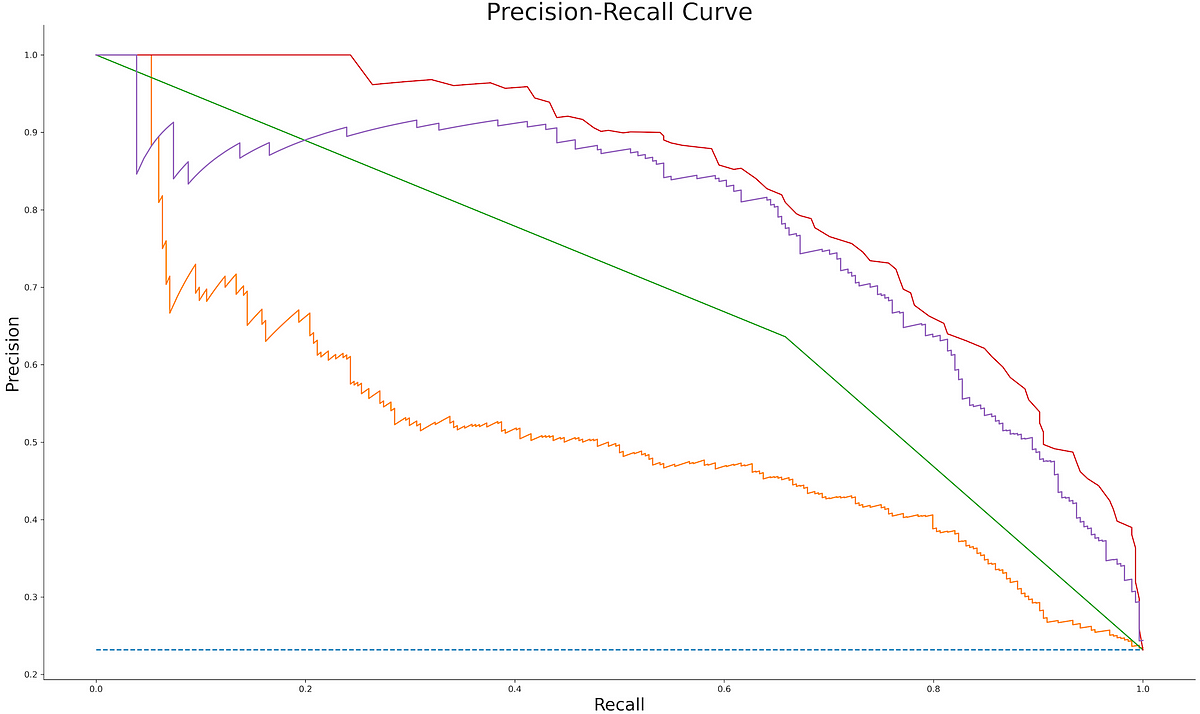
\includegraphics[width=0.6\textwidth]{prcurve.png}
  \caption{PR曲线 \label{fig:prcurve}}
\end{figure}





\subsection{多分类模型}


\section{回归问题的评估指标}